\documentclass[12pt]{article}
\usepackage{hyperref}
\usepackage{listings}
\usepackage[margin=1in]{geometry}
\usepackage{enumitem}
\usepackage{multicol}
\usepackage{array}
\usepackage{titlesec}
\usepackage{helvet}
\renewcommand{\familydefault}{\sfdefault}
\usepackage{amsmath}     % For math equations
\usepackage{amssymb}     % For advanced math symbols
\usepackage{amsfonts} % For math fonts
\usepackage{gvv}
\usepackage{esint}
\usepackage[utf8]{inputenc}
\usepackage{graphicx}
\usepackage{pgfplots}
\pgfplotsset{compat=1.18}
\titleformat{\section}{\bfseries\large}{\thesection.}{1em}{}
\setlength{\parindent}{0pt}
\setlength{\parskip}{6pt}
\usepackage{multirow}
\usepackage{float}
\usepackage{caption}


\begin{document}

\section*{Problem 5.3.26}
For what value of $k$, does the system of linear equations
\begin{align}
2x + 3y = 7, \qquad (k-1)x + (k+2)y = 3k
\end{align}
have an infinite number of solutions?

\section*{Input Variables and Vectors}
\begin{center}
\begin{table}[H]
\centering
\begin{tabular}{|c|c|c|}
\hline
\textbf{Symbol} & \textbf{Description} & \textbf{Value/Expression} \\
\hline
$x,y$ & Unknown variables & Real numbers \\
$k$ & Parameter in system & To be determined \\
$\vec{x}$ & Unknown vector & $\myvec{x \\ y}$ \\
$A$ & Coefficient matrix & $\myvec{2 & 3 \\ k-1 & k+2}$ \\
$\vec{b}$ & RHS vector & $\myvec{7 \\ 3k}$ \\
$[A|b]$ & Augmented matrix & $\myvec{2 & 3 & 7 \\ k-1 & k+2 & 3k}$ \\
\hline
\end{tabular}
\caption{}
\label{}
\end{table}
\end{center}

\section*{Solution}
\begin{align}
\myvec{2 & 3 \\ k-1 & k+2}\vec{x} &= \myvec{7 \\ 3k}, \quad 
\text{where } \vec{x} = \myvec{x \\ y}.
\end{align}

\begin{align}
\text{The augmented matrix is } 
\myvec{2 & 3 & 7 \\ k-1 & k+2 & 3k}.
\end{align}

\begin{align}
R_2 &\to R_2 - \tfrac{k-1}{2}R_1 \\[6pt]
\myvec{2 & 3 & 7 \\ k-1 & k+2 & 3k}
&\to 
\myvec{2 & 3 & 7 \\ 0 & (k+2) - \tfrac{3}{2}(k-1) & 3k - \tfrac{7}{2}(k-1)}.
\end{align}

\begin{align}
&= \myvec{2 & 3 & 7 \\ 0 & \tfrac{-k+7}{2} & \tfrac{-k+7}{2}}.
\end{align}

\begin{align}
\text{For infinite solutions: } 
\operatorname{rank}(A) &= \operatorname{rank}([A|b]) < 2.
\end{align}

\begin{align}
\tfrac{-k+7}{2} &= 0 \quad \Longrightarrow \quad k=7.
\end{align}

\begin{align}
\text{When } k=7,\quad
\myvec{2 & 3 & 7 \\ 0 & 0 & 0},
\end{align}

\begin{align}
\operatorname{rank}(A) &= \operatorname{rank}([A|b])=1 < 2.
\end{align}

\begin{align}
\therefore \quad \text{The system has infinitely many solutions when } 
\boxed{k=7}.
\end{align}

\begin{figure}[H]
    \centering
    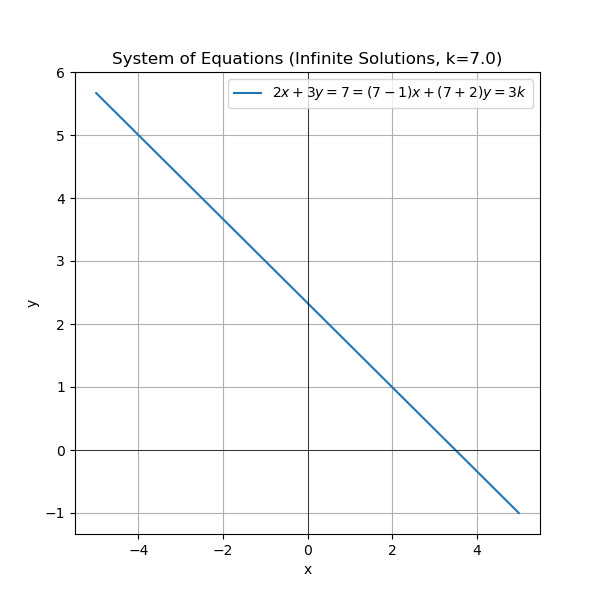
\includegraphics[width=0.9\columnwidth]{figs/infsols.png}
    \caption{}
    \label{fig:placeholder}
\end{figure}


\end{document}
